\documentclass{article}
\usepackage[T2A]{fontenc}
\usepackage[utf8]{inputenc}
\usepackage[english, russian]{babel}
\usepackage[left=3cm,right=3cm,top=2cm,bottom=1.5cm]{geometry}
\usepackage{fancyhdr}
\usepackage{graphicx}
\usepackage{tikz}
\usepackage{amsmath}
\usepackage{hyperref}
\renewcommand{\labelenumii}{\arabic{enumi}.\arabic{enumii}.}
\usetikzlibrary{trees}
\tikzstyle{level 1}=[level distance=2.5cm, sibling distance=4cm]
\tikzstyle{level 2}=[level distance=2.5cm, sibling distance=2cm]
\graphicspath{{pictures/}}
\DeclareGraphicsExtensions{.pdf,.png,.jpg}
\pagestyle{fancy}
\fancyhf{}
\fancyfoot[R]{\thepage}
\renewcommand{\headrulewidth}{0pt}
\renewcommand{\footrulewidth}{0pt}
\renewcommand{\labelitemii}{$\circ$}
\renewcommand{\labelitemi}{$\bullet$}
\usepackage{tempora} %Times New Roman alike
\usepackage{newtxmath} 



\date{\today}

\begin{document}
\thispagestyle{empty}
\begin{center}
    \LARGE\textbf{МИНОБРНАУКИ РОССИИ\\
        САНКТ-ПЕТЕРБУРГСКИЙ ГОСУДАРСТВЕННЫЙ\\
        ЭЛЕКТРОТЕХНИЧЕСКИЙ УНИВЕРСИТЕТ\\
        "ЛЭТИ"\ ИМ. В.И.УЛЬЯНОВА(ЛЕНИНА)\\
        Кафедра МО ЭВМ}\\[6cm]
    \Large\textbf{ОТЧЁТ}\\[0.2cm]
    \Large\textbf{по курсовой работе}\\[0.1cm]
    \Large\textbf{по дисциплине <<Алгоритмы и структуры данных>>}\\[0.1cm]
    \Large\textbf{Тема: Демонстрация работы пирамиды.}\\[5cm]
\end{center}
\Large{Студент гр. 1304 \qquad \qquad \quad \underline{\hspace{4cm}} \qquad \qquad Мусаев А.И.}\\[0.5cm]
\Large{Преподаватель \qquad \qquad \qquad \underline{\hspace{4cm}} \qquad \qquad Шевская Н.В.}\\[1cm]
\begin{center}
    Санкт-Петербург\\
    2022
\end{center}
\newpage
\begin{center}
    \textbf{Задание на курсовую работу}
\end{center}

Студент: Мусаев А.И.

Группа: 1304

Тема работы: Демонстрация работы пирамиды\\

Реализовать следующие алгоритмы на основе пирамиды:

\begin{itemize}
    \item Вставка элемента
    \item Удаление наименьшего элемента
    \item Поиск элемента
    \item Пирамидальная сортировка
\end{itemize}.\\

Содержание пояснительной записки:

\begin{itemize}
    \item Введение
    \item Основные теоретические положения
    \item Реализация программы
    \item Тестирование
    \item Заключение
\end{itemize}

\vspace{1cm}

Дата выдачи задания: 25.10.2022

Дата сдачи работы: **.**.2022

Дата защиты работы: **.**.2022\\

\vspace{3cm}

\Large{Студент гр. 1304 \qquad \qquad \quad \underline{\hspace{4cm}} \qquad \qquad Мусаев А.И.}\\[0.5cm]

\Large{Преподаватель \qquad \qquad \qquad \underline{\hspace{4cm}} \qquad \qquad Чайка К.В.}\\[1cm]

\newpage

\begin{center}
    \textbf{АННОТАЦИЯ}
\end{center}

В данной курсовой работе была реализована программа, имеющая следующий функционал на основе пирамиды:

\begin{itemize}
    \item Вставка элемента
    \item Удаление наименьшего элемента
    \item Удаление наибольшего элемента
    \item Поиск элемента
    \item Пирамидальная сортировка
\end{itemize}
\newpage

\begin{center}
    \textbf{НАВИГАЦИЯ ПО ПОЯСНИТЕЛЬНОЙ ЗАПИСКЕ}
\end{center}

\tableofcontents{}

\newpage

\begin{center}
    \textbf{ВВЕДЕНИЕ}
\end{center}

Целью данной работы является разработка программы, которая имеет функционал по работе со структурой данных пирамида.

Программа должна получать исходные данные из командной строки и выполнять поставленные ей задачи.
Кроме того, программа должна демонстрировать выполняемые ею процессы.

Для реализации данной программы предстоит решить следующие задачи:

\begin{itemize}
    \item Изучить структуры данных пирамида
    \item Изучить операции с пирамидой
    \item Изучить пирамидальную сортировку
    \item Реализовать удобный для пользователя интерфейс, так как работа программы демонстрируется пользователю
    \item Реализовать демонстрацию, понятную для пользователя
\end{itemize}

\newpage

\section{Основные теоретические положения}

\subsection{Что такое пирамида?}

Пирамида или куча - абстрактная структура данных, поддерживающая следующие операции:

\begin{enumerate}
    \item Нахождение минимума
    \item Удаление минимума
    \item Добавление нового элемента в кучу
\end{enumerate}

Другое название, лучше отражающее функциональность — очередь с приоритетами.

Кучи используются во многих алгоритмах. Например, кучи используются в алгоритмах поиска кратчайшего пути, а также с помощью кучи можно проводить сортировку (путём превращения массива в кучу, а кучу в отсортированный массив).

Для кучи всегда выполнены условия:

\begin{enumerate}
    \item Значение в любой вершине не больше, чем значения её потомков
    \item У любой вершины не более двух сыновей
    \item Слои заполняются последовательно сверху вниз и слева направо, без «дырок»
\end{enumerate}

Заметим, что двоичная куча строится неоднозначно: например, значения сыновей, которые являются листами, всегда можно менять местами. Фиксирована только сама структура и предикат «родитель не больше детей».

\begin{figure}[h]
    \centering
    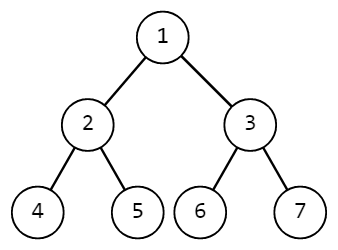
\includegraphics[width=0.4\linewidth]{1.png}

    \caption{Куча для минимума}

    \label{fig:mpr}

\end{figure}

Обозначим высоту дерева как $h$. Так как куча всегда состоит из нескольких слоев заполненных полностью и одного заполненного частично, и каждый следующий слой содержит в два раза больше вершин, чем предыдущий, то высота дерева будет $\theta(log n)$.

Как и любая очередь с приоритетами, двоичная куча должна уметь выполнять операции:

\begin{enumerate}
    \item Нахождение минимума за $O(1)$.
    \item Удаление минимума за $O(h)$.
    \item Добавление нового элемента в кучу за $O(h)$.
\end{enumerate}

\subsection{Как осуществляется вставка элемента?}

Чтобы вставить элемент в дерево, мы выполняем следующий алгоритм:

\begin{enumerate}
    \item Дописывем элемент на нижний уровень в крайнем правом пустом ребёнке.
    \item Сравниваем элемент с родительским, если они расположены в верном порядке, останавливаемся.
    \item Иначе меняем с родительским и переходим к предыдущему шагу.
\end{enumerate}

2 и 3 шаги алгоритма называют просеиванием вверх.

Ассимптотика такого алгоритм $O(h)$, так как мы проходим все уровни дерева, а высота дерева, как мы ввели, равна $h$.

\begin{figure}[h]
    \centering
    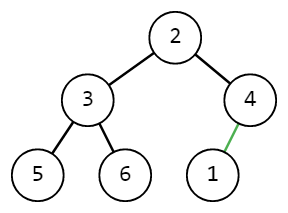
\includegraphics[width=0.3\linewidth]{2.png}
    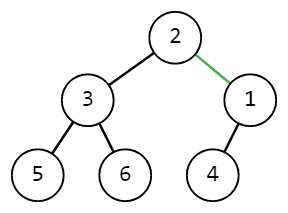
\includegraphics[width=0.3\linewidth]{3.png}
    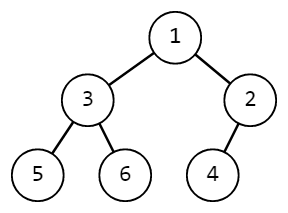
\includegraphics[width=0.3\linewidth]{4.png}
    \caption{Пример работы алгоритма вставки}
    \label{fig:mpr}
\end{figure}

\subsection{Удаление наименьшего элемента}

Процедура удаления корня из кучи с сохранением свойства кучи выглядит следующим образом:

\begin{enumerate}
    \item Заменяем корень кучи последним элементом на последнем уровне.
    \item Сравниваем новый корень с его дочерними элементами; если они расположены в правильном порядке, останавливаемся.
    \item Если нет, заменяем элемент одним из его дочерних элементов и возвращаемся к шагу 2. 
\end{enumerate}

2 и 3 шаги называют просеиванием вниз.

Ассимптотика такого алгоритм тоже $O(h)$, так как мы проходим все уровни дерева.

\begin{figure}[h]
    \centering
    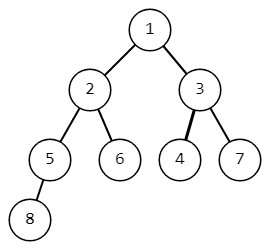
\includegraphics[width=0.3\linewidth]{5.png}

    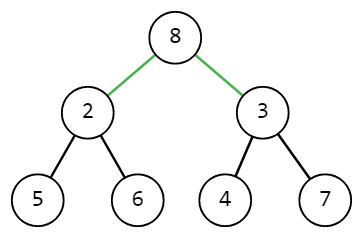
\includegraphics[width=0.3\linewidth]{6.png}
    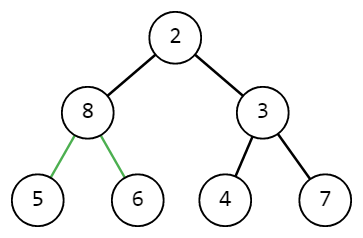
\includegraphics[width=0.3\linewidth]{7.png}
    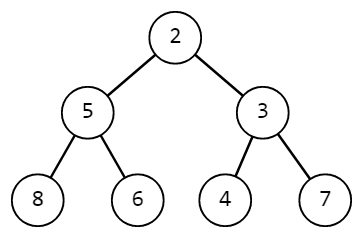
\includegraphics[width=0.3\linewidth]{8.png}
    \caption{Пример работы алгоритма удаления минимального}
    \label{fig:mpr}
\end{figure}

\subsection{Удаление наибольшего элемента}

Удаление наибольшего рассматриваем для мин-кучи, так как для макс-кучи оно описано в предыщем пункте.

\begin{enumerate}
    \item Пробегаемся по нижне половине дерева.
    \item Находим максимум.
    \item Ставим на место максимума последний лист.
    \item Просеиваем новое значение вверх.
\end{enumerate}

Ассимптотика такого алгоритм - $\frac{n}{2}$ + $log n$, то есть $O(n)$, так как пробежаться по нижней половине дерева - это $\frac{n}{2}$ операций, а просеить вверх - это $log n$ операций.

\begin{figure}[h]
    \centering
    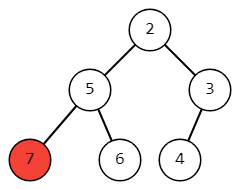
\includegraphics[width=0.3\linewidth]{9.png}
    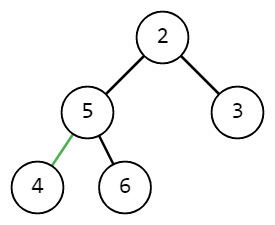
\includegraphics[width=0.3\linewidth]{10.png}
    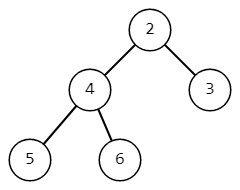
\includegraphics[width=0.3\linewidth]{11.png}
    \caption{Пример работы алгоритма удаления максимального}
    \label{fig:mpr}
\end{figure}

\newpage

\subsection{Поиск элемента}

К сожалению, куча не рассчитана на оптимальный поиск элемента, поэтому поиск происходит за $O(n)$, нам нужно просто пройтись по все элементам дерева.

\subsection{Пирамидальная сортировка}

В пирамидальной сорировке такой алгоритм:

\begin{enumerate}
    \item Построить макс-кучу из входного массива.
    \item Извлечь максимальный элемент и переставить его в конец массива.
    \item Вернуться к шагу 1 с массивом размером на 1 меньше.
\end{enumerate}

Ассимптотика такого алгоритма $O(n*log n)$, так как мы извлекаем $n$ элементов, а после каждого извлечения идёт просеивание вниз за $log n$.

Построение кучи работает так:

Мы запускаем рекурсивную функцию, которая наведёт порядок сначала на самых нижних уровнях кучи и дойдёт так до корня дерева. Так мы получим верное дерево и начнём извлекать элементы.

\newpage

\section{Реализация программы}

\subsection{Файл main}

Здесь происходит взаимодействие с пользователем: тут происходит считывание команд от пользователя и проверка входных данных, которые подаёт пользователь.

Сначала происходит считывание максимального размера дерева, так как куча хранится на основе массива.
Затем происходит создание кучи и вывод правил пользования.

\subsection{Файл Heap}

Хранить кучу будем в виде массива, где у корня индекс равен 0, а у вершины $k$ индексы ее детей равны $2k+1$ и $2k + 2$.

В этом файле хранится класс кучи. В нём есть следующие методы:

\begin{enumerate}
    \item get\_parent(index) - метод, возвращающий индекс родителя, то есть просто \texttt{return (index - 1) // 2}
    \item get\_left\_child, get\_right\_child - методы, возвращающие индексы детей по формуле, написанной выше.
    \item insert - добавление элемента в дерево. (пункт 1.2)
    \item extract\_min - удаление минимального. (пункт 1.3)
    \item sift\_up - просеивание вверх.
    \item sift\_down - просеивание вниз.
    \item str - преобразование массива в строку.
    \item extract\_max - удаление наибольшего. (пункт 1.4)
    \item search - поиск элемента (пункт 1.5)
\end{enumerate}

\subsection{Файл Sort}

В этом файле хранятся функции, выполняющие сортировку пирамидой.

Функция heapify(a, n, index) выполняет правильную расстановку элементов в дереве, то есть:

\begin{enumerate}
    \item Находит индексы правого и левого ребёнка поданного узла.
    \item Находит максимальный элемент из 3: из родителя, правого и левого ребёнка.
    \item Если один из детей больше родителя, меняем их местами, вызываем функцию heapify от нового индекса поданного элемента, чтобы проверить, что, когда мы навели порядок на нынешнем уровне, не сломали всё уровнем ниже.
\end{enumerate}

Функция heap\_sort(a, flag\_want) сначала наводит порядок в массиве (превращает его в дерево): она вызывает heapify на всех уровнях, кроме последнего, на последнем не вызывается, так как у них нет детей.

После наведения порядка вызывается цикл, который извлекает максимальный элемент, переставляет его в конец массива, наводит порядок в куче на один меньше и делает ещё раз то же самое, пока не дойдёт до 0 элемента в массива.

\subsection{Файл visual}

Этот файл рисует дерево. 

В нём есть:

\begin{itemize}
    \item Класс узел (TreeNode), который может хранить в себе значение, ссылку на левого и ссылку на правого ребёнка. 
    \item Функция deserialize создаёт из массива дерево, хранящееся через класс TreeNode и возвращается корень этого дерева
    \item Функция drawtree хранит в себе несколько функций:
        \begin{itemize}
            \item height - находит высоту дерева
            \item jumpto - переносит исполнителя turtle на нужные координаты
            \item draw - вывод самого узла и его детей
        \end{itemize}
        Это всё вспомогательные функции для того, чтобы делать основную работу вывода дерева. Сначала находим высоту дерева. Черепаха переходит на нужные координаты и рекурсивно рисует дерево.
\end{itemize}


\newpage

\section{Тестирование}


\newpage

\section{Заключение}

В ходе данной курсовой работы была изучена структура данных пирамида.

Реализованная программа принимает на вход комманды, исходя из которых проводит демонстрацию работы пирамиды.

В ходе курсовой:
\begin{itemize}
    \item Был изучен теоретический материал по пирамиде
    \item Был разработан и реализован программный код
    \item Было проведено тестирование программы
\end{itemize}

\newpage

\section{Список используемых источников}

\begin{itemize}
    \item https://shkolkovo.online
    \item https://ru.algorithmica.org
    \item https://stackoverflow.com
    \item https://en.wikipedia.org/wiki/Heapsort
\end{itemize}

\end{document}